\documentclass[a4paper, 11pt]{article}
\usepackage{fullpage, hyperref, color, amsmath, listings, graphicx, wrapfig} % changes the margin

\usepackage{graphicx}
\begin{document}
%Header-Make sure you update this information!!!!

\title{Procedurally Producing Pairs of Paintings \\ \medskip
\large{CS 0451 Final Project Report}}
\author{Cole Ellison, Hans Goudey, Henry Swaffield}
\maketitle

\newcommand{\link}[2]{\color{blue}\href{#1}{#2}\color{black}}
\newcommand{\confusion}[4]{
  \medskip
  \begin{tabular}{|c|c|}
    \hline
    #1 & #2 \\
    \hline
    #3 & #4 \\
    \hline
  \end{tabular}
  \medskip
}

\section{Links}
\begin{itemize}
  \item \link{http://www.cs.middlebury.edu/~crellison/cs451/}{website}
  \item \link{https://github.com/crellison/finalML}{github}
\end{itemize}

\section{Introduction}

Our goal was to use \link{https://www.kaggle.com/c/painter-by-numbers}{a kaggle dataset of paintings } to build a model that can predict whether two paintings were created by the same artist. One of the best ways to tackle this problem is to use a Siamese network. Siamese networks use two smaller and identical networks to extract features from their two inputs, and then use a comparison or distance function to tell how similar these two sets of features are. The similarity of feature values in the generated feature space indicates whether the two images are from the same class.

Another approach would be to use a classifier for every artist in the dataset. The problem with this approach is that it does not scale to artists not included in the training set or artists who do not have enough paintings in the dataset to build a robust classifier. Theoretically, a Siamese network can take in two images it has never seen before and output the probability of them sharing some property—an artist, for example. As our experimentation will show, a Siamese NN can be trained on one type of data, and still be useful on another type of data that it has not previously seen, and example of zero-shot learning.

\section{Experimental Setup}

\subsection{Description of Datasets}

In addition to building a common artist recognizer for the painting dataset, experimentation led us to build another siamese model that could run on \link{https://www.kaggle.com/zalando-research/fashionmnist}{MNIST fashion data} and the MNIST handwritten digit dataset, and also a classifier for the same data set, both using convolutional neural nets. These smaller datasets allowed for rapid iteration and debugging on less powerful machines. Training the painting dataset on a standard macbook proved too time intensive to validate the construction of our Siamese convolutional neural network.

\subsection{Painter by Numbers Dataset}

The painting kaggle dataset contains ~79,000 images of paintings with a median size of approximately $800 \times 800$ pixels and the largest images being more than 200MB. These images are not square, so some preprocessing is required before they can be fed into a vanilla Siamese CNN. Though we looked into some auto-squaring layers and other preprocessing options, they proved either too confusing or infeasible in the time we had. 

\subsection{MNIST Fashion and Digit Datasets}

The MNIST datasets follow a standard $28 \times 28$ pixel layout of single channel color. Their small size allowed us to fit the entire training set in memory without issue, leading to a more simplified workflow and easier validation of our proof of concept.


\subsection{Siamese Network Input Shape}

A siamese neural network’s input are pairs of inputs, with each input of the pair going to one of the twin sub-networks. As we explored siamese nets, we learned that our training data would be a list of image pairs generated from the original set of images. We went about this task similarly for the MNIST and painting datasets.

\subsection{Data Generation}

One consideration related to the tradeoff between having more data, but not skewing it towards pairs with non-matching labels. Because each painter represents a very small portion of our painting dataset, there are fewer common-artist pairs compared to the number of possible different-artist pairs. The same problem applies to the mnist-datasets. Rather than generate all possible image pairs of paintings, fashion items, or digits we decided to limit the amount we produce so that there would be a roughly 50\%--50\% split between the number of outputs where $y=1$ or $y=0$. The goal of this 50-50 split is to make the model just as good at recognizing each type of pair, even though same-artist pairs could end up being less common in any real-life application.

Our cross validation set is a subset of the training pairs generated by the above method. We used straightforward prediction accuracy as our metric of evaluation. For our cross validation experimentation we do not consider confidence in the predictions, though the optimization objective is to maximize the distance in the feature space output by the sub-nets.

\subsection{Generating Batches for the Painting Network}

Normally, to train a keras network you use a function that takes in the entire dataset in one numpy array and breaks down the training into epochs and batches. However, with our painting image dataset, this proved impossible. Although the images were less than 2GB compressed in JPEG format, with over 9 million training pairs, even after reducing the original image size to $200 \times 200$, this array would take up way too much memory:

\[
  (9 000 000 \times 2) \times (200 \times 200) \times 4_\text{float32} \times 3_\text{channels}  \text{ bytes} = 8.64 \text{ terabytes}
\]
\\
Because of this, we had to build a function to generate smaller batches for the painting Siamese network. Our \texttt{get\_batch} function generates these batches, 4D numpy arrays of shape (Batch size, height, width, channels), and the network trains on each batch and generates the next one. We were able to choose the image dimension on the fly, and varied them along with the batch size to fill the 8GB of GPU memory as much as possible.

\subsection{Problems with the Output of the Models}

Our model outputs the distance between the generated feature sets from the two images. The maximum euclidean distance can depend on the number of dimensions in the space it is comparing. This is one problem we didn’t end up completely solving. Ideally we transform this distance output into a probability programmatically by choosing the median or mean of the distance outputs as the threshold between a prediction of 1 or 0, but because of time constraints, and having larger problems elsewhere in the code, the threshold we used was 0.5, based on an assumption that the output of the distance function should be between 0 and 1.

\subsection{Training with a GPU}

\begin{wrapfigure}{r}{5.5cm}
  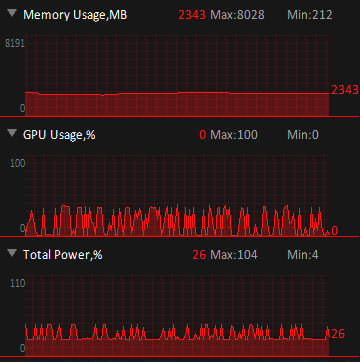
\includegraphics[width=5.5cm]{GPU.png}
\end{wrapfigure}
One time consuming process was setting up the GPU for training our model much faster. Keras uses different backends to make use of GPU acceleration, \link{http://www.deeplearning.net/software/theano/}{Theano}, \link{https://www.tensorflow.org/}{Tensorflow}, and \link{https://github.com/Microsoft/CNTK}{CNTK}. We ran into problems with the installation of Theano and Tensorflow, but the installation of CNTK worked well. First it required the installation of NVidia \link{https://developer.nvidia.com/cuda-zone}{CUDA} for GPU acceleration, then the installation of \link{https://developer.nvidia.com/cudnn}{CuDNN}, a library for the implementation of GPU accelerated neural networks. Using the GPU significantly sped up our training, and we were able to monitor the GPU usage to make sure our model was training and diagnose memory issues. 

\subsection{Standalone CNN Application for practice} 

While determining which sub-network architecture to use for our main painting Siamese network, we built a convolutional NN to run on the fashion data. This network performed a basic neural network classification of the fashion data into the 10 categories of images. We designed two different CNNs for the task, one for use on the GPU and another to test with on our laptops. With the fashion dataset, we were able to rapidly put together a working CNN that predicted the clothing category with 87\% accuracy after only an hour of work. Further fine tuning of parameters put us at over 90\% accuracy (results included below). With a working subnet, we now felt more confident that our overall implementation was working, as prediction a classification should translate with relative ease to prediction of similarity. On immediate testing, we found that the Siamese implementation achieved 84--86\% accuracy, which is better than just using two classifiers in isolation ($0.91^2 = 0.82 $).

\section{Results}

\subsection{Arrangement of the Confusion Matrix}

For all results, the confusion matrix is arranged as shown below.

\confusion{true negative}{false positive}{false negative}{true positive}

\subsection{Standalone CNN Fashion Classifier}

We tested a standalone CNN classifier on fashion mnist data, getting a max cross validation accuracy of 91\%. According to \link{http://fashion-mnist.s3-website.eu-central-1.amazonaws.com/}{a site containing benchmark dat}a for various machine learning approaches to the fashion MNIST dataset, this performance outperforms traditional classifiers, such as SVCs and Logistic Regression.

\subsection{Siamese Model for Dashion and Digit Data}

Our siamese classifier for fashion data got an accuracy of 86\% on the cross validation set. Once again, we generated a very large number of pairs (~120,000), and so we have confidence in the statistical significance of this result. 

The confusion matrix for our Siamese Classifier of MNIST Fashion (accuracy: 0.86066):

\confusion{9303}{2097}{687}{7893}

Our Siamese classifier for digit data performed better, scoring an accuracy of 93\% on the cross validation set. Once again, as shown in the following confusion matrix, this included many thousands of test examples, and so we have confidence in the statistical significance of the result. It is exciting to see that this architecture is performing better than if we had used two vanilla-cnn’s and then compared their outputs directly (.91 error $\times$ .91 error = .8281), because it indicates the Siamese architecture is actually optimizing for differentiating classes, as we hoped it would.

The confusion matrix for our Siamese Classifier of MNIST Digits (accuracy: 0.93681).

\confusion{8834}{1050}{76}{7860}

\subsection{Siamese Model Applied to Different Data: Zero-Shot-Learning}

Perhaps one of the most interesting characteristics of Siamese Neural nets is that they are not directly classifying the paintings, digits, or clothing pictures. They are classifying pairs, and determining what characteristics images that fall into the same class, may have. This is why a pair of paintings by an artist never seen before by a trained Siamese network could still be recognized as coming from the same artist.

We explored that type of scenario with our lighter-weight Siamese Nets, and the results appear significant for at least one, and also somewhat surprising.

Training a Siamese net to determine whether two digits are the same produces a Siamese net that is still useful at determining whether two fashion images are in the same class:

The confusion matrix for our Siamese Classifier trained on MNIST Digits and tested on MNIST Fashion (accuracy: 0.615766):

\confusion{7569}{5256}{2421}{4734}

While the accuracy is much lower than if we had trained on actual fashion images, it is fascinating to see that it can still determine whether two images are the same item, because \textit{the network that produced those results never previously saw fashion data}.

Interestingly, when the experiment is reversed, the results are less impressive, getting an accuracy of 54\%. This initially surprised us because differentiating digits seems to be an easier problem, as our previous results would suggest (our Siamese net for digit differentiation did the better than it’s fashion-focused counterpart). 

The confusion matrix for our Siamese Classifier trained on MNIST Fashion and tested on MNIST Digits (accuracy: 0.615766):

\confusion{7017}{6254}{1893}{2656}

\subsection{Siamese model for painting data}

We ended our investigation into the painting Siamese network somewhat unsatisfied. We ended up with code that created a model weights file to load later and outputted the accuracy of that model. A third of the time, this model would work. After seeing 16,000 examples, it had a 57\% accuracy. However, with no code changes, the other two thirds of our training runs would create models that didn’t work at all, usually by outputting the same prediction for every test example. After testing many times, this behavior was the single most perplexing challenge we faced, as there were no changes occurring in the python file, especially because it made more substantial training-runs infeasible.

\section{Conclusions}

Although the situation of temporal failures of our painting Siamese network was frustrating, a 57\% accuracy after just a very small fraction of the dataset is promising, and suggests that more training could produce a strong model. But with code that only works some of the time, it’s hard to commit a long time to training.

However, our results for the other networks were much better and show that we gained an understanding for how to build convolutional neural networks, as well as combine them to form more complicated models.

\section{Acknowledgements}

We would like to thank the communities at Kaggle and Keras for developing and maintaining interesting datasets and the powerful tools that we utilized to complete this project.

Specifically, we would like to thank Kiri Nichol (A.K.A Small Yellow Duck) for organizing the competition that inspired this project, and for providing an implementation of a Siamese net. Viewing his architectures made the overall ideas behind Siamese Neural Nets much more clear, and we used his \link{https://github.com/small-yellow-duck/kaggle_art/blob/master/mnist_siamese_cnn.py}{euclidean distance functions}, as well.


\newpage
\begin{thebibliography}{9}

  \bibitem{Bouma} Bouma, Soren. ``One Shot Learning and Siamese Networks in Keras.'' Neural Tinkering. 29 March 2017. (https://sorenbouma.github.io/blog/oneshot/)
  
  \bibitem{Comp} Computerphile. ``Neural Network that Changes Everything.'' 20 May 2016. \newline (https://www.youtube.com/watch?v=py5byOOHZM8)

  \bibitem{Des} Deshpande, Adit. ``A Beginner's Guide To Understanding Convolutional Neural Networks Part 2.'' 29 July 2016. (https://adeshpande3.github.io/A-Beginner\%27s-Guide-To-Understanding-Convolutional-Neural-Networks-Part-2/)

  \bibitem{Karn} Karn, Ujjwal. ``An Intuitive Explanation of Convolutional Neural Networks.'' The Data Science Blog. 11 Aug 2016. (https://ujjwalkarn.me/2016/08/11/intuitive-explanation-convnets/)

  \bibitem{Wiki} Wikipedia. ``Convolutional Neural Network.'' 2017. \newline(https://en.wikipedia.org/wiki/Convolutional\_neural\_network)

  \bibitem{Parajuli} Parajuli, Nripesh. ``Siamese.'' GitHub. 23 Aug 2017. \newline(https://github.com/ascourge21/Siamese)
\end{thebibliography}

\end{document}